\section{Analysis and Results}
\label{sec:description_3}

When defining our game space $\Gamma$ in Section \ref{subsec:pirates_initialstate} we defined a number of variable parameters, such as: the entanglement coefitient $\gamma$; the coin distributions $\alpha_{ij}$; the strategies $\mathcal{U}_{j}$ that the players might use (restricting the operator space $\mathsf{SU}(2)$). 

According to \cite{Du} when the entanglement is maximal, $\mathcal{U}(\pi, 0)$ is the optimal counter-strategy for $C$ (represented by the identity marix), $\mathcal{U}(0, \frac{\pi}{2})$ is the optimal counter strategy for $\mathcal{U}(\pi, 0)$, $D$ becomes the optimal counter-strategy for $\mathcal{U}(0, \frac{\pi}{2})$, and $C$ becomes an optimal counter strategy for $D$.

\subsection{$2$ Player Game}
\label{subsec:2playergame}

We simulated the Pirate Game for $2$-players according to the rules defined for our quantum model in Section . The simulation can be consulted for reference in Appendix \ref{ap:d}. The classical sub-game with $2$-players can be represented in Table \ref{tab:classico2jogadores_analise}.

\begin{table}[h]
\begin{center}
\begin{centering}
\begin{tabular}{ccc}
\hline 
  & Player 2: C & Player 2: D\tabularnewline
\hline 
Player 1: C & (100, 0) & (100, 0)\tabularnewline
Player 1: D & (100, 0) & (-200, 100.5)\tabularnewline
\hline 
\end{tabular}

\par\end{centering}
\caption{Representation of the $2$ player sub-game in normal form.}
\label{tab:classico2jogadores_analise}
\end{center}



\subsection{$3$ Player Game}
\label{subsec:3playergame}


\subsubsection{The captain proposes: $(99, 0, 1)$}
\label{subsubsec:3playergame99}

The move $(C_1,D_2,C_3,C_4,D_5)$ with a proposal of $(\alpha_{1}, \alpha_{2}, \alpha_{3}) =(99, 0, 1)$ represents Nash Equilibrium of the classic Pirate Game (for $3$ players). In the classical version, when the players chose at least $2$ operators $Cooperate$ on the initial proposal the game ends right away, and the first proposal, made by player $1$, is accepted ($Accepted 1$ or $A_{1}$).

After the players make their strategic moves and the disentangle operator $\mathcal{J}^{\dagger}$ is applied, and the payoff functionals are calculated given the final state. The final state will be calculated as shown in Equation \ref{eq:piratas_final_move_23}.

\begin{equation}
\vert\psi_{fin}\rangle=\otimes_{i=1}^{3}\otimes_{j\in\xi^{-1}(i)}\mathcal{U}_{j}\vert\psi_{ini}(\gamma)\rangle
\label{eq:piratas_final_move_23}
\end{equation} 

As expected from the problem definition when players use only classical strategies the entanglement coefitient will not affect the final expected utilities ($[ \mathcal{J} , C \otimes D \otimes C \otimes C \otimes D ] = 0 $).
An example of this behaviour is shown in Figure \ref{fig:pg_3players_99_0_1}, where we measure the probability $A_{1}$ (first proposal is accepted), $A_{2}$, and $R_{2}$, with diffent entanglement levels ($\gamma= \{ 0 , \frac{ \pi}{4}, \frac{\pi}{2} \} $).

\begin{figure}[h]
\centering 
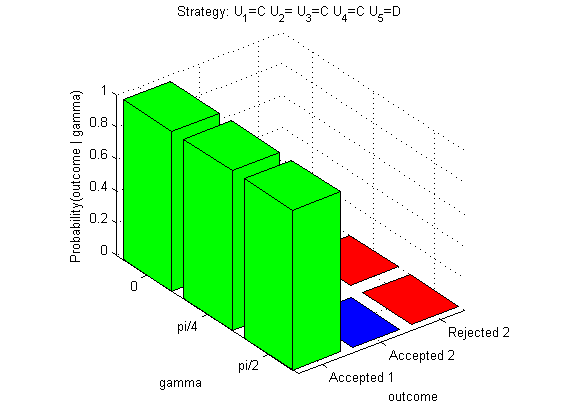
\includegraphics[scale=0.80]{Figures/1.5qubit/CDCCD.png}
\caption{When player play classical strategies the entanglement will not affect the final result. }
\label{fig:pg_3players_99_0_1}
\end{figure}

When each player chooses an operator from the set $O = \{ \mathcal{U} ( \theta , 0) , \theta \in (0, \pi) \}$ and $\gamma=0$ we have an equivalent to the classic mixed strategies. However for $\gamma >0$ the $\mathcal{U} ( \theta , 0)$ may present an interference behaviour that is innerentely quantum. This effect is shown in Figures \ref{fig:pg_3players_99_0_1:2} and \ref{fig:pg_3players_99_0_1:2}, allowing us to understand the difference between the Bit-flip operator $D$ and $\mathcal{U} ( \pi , 0)$.



\begin{figure}[h]
\centering 
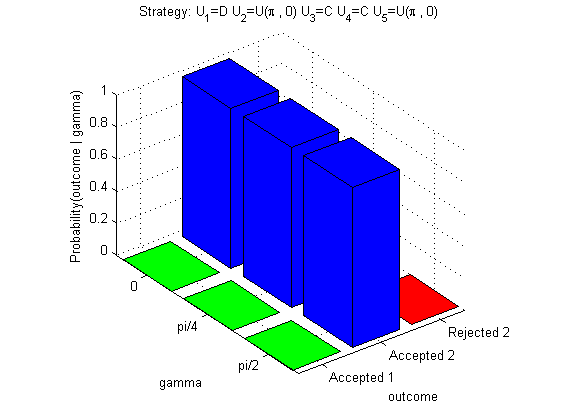
\includegraphics[scale=0.80]{Figures/1.5qubit/DUpi0CCUpi0.png}
\caption{Players use the operators . }
\label{fig:pg_3players_99_0_1:2}
\end{figure}

\begin{figure}[h]
\centering 
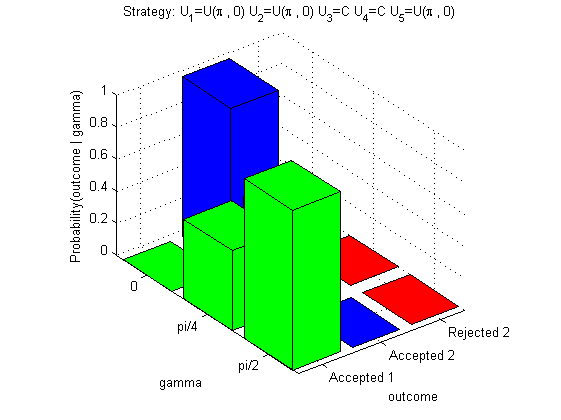
\includegraphics[scale=0.80]{Figures/1.5qubit/Upi0Upi0CCUpi0.png}
\caption{Unlike with the Bit-flip operator $D$, $\mathcal{U} (\pi, 0)$ is affected by the entanglement coeficient $\gamma$ in this case. }
\label{fig:pg_3players_99_0_1:3}
\end{figure}




























\begin{comment}

In a classical game the best response for player $1$ is to cooperate. In this quantum version depending of the parameter $\gamma$, the strategy that produces the most favourable outcome changes. However if the first proposal is rejected and player $1$ voted in favour (using the $C$ operator), we get to a final sub-game where the parameter $\gamma$ won't influence the expected utility; these results for this can be consulted on Appendix \ref{ap:d}, Section \ref{ap:d:CDD99}. Table \ref{repro:3} displays a particular outcome of the sub-game generated when the players chose the operators $CDD$ in the first stage ($CD$); it shows the expected utility when player $2$ accepts her proposal, and player $3$ rejects. 


This happens due to the nature of the game, more specifically the way we calculate our expected utility for each player, which is described in Section \ref{subsec:pirates_utility}, Equation \ref{eq:pirates_payoff32}. The sum of the probability for the system being on states $\vert CCD\rangle$ or $\vert CDC\rangle$ is constant ($\frac{1}{2}$), this also happens with the sum of the probability of the system being on state $vert DCD\rangle$ or $\vert DDC\rangle$.

However the parameter $\gamma$ affects the probability of the system being measured in a determined state, as in Table \ref{repro:3}.

 \begin{table}[h]
\begin{center}
\begin{tabular}{cc}
  c)\putindeepbox[7pt]{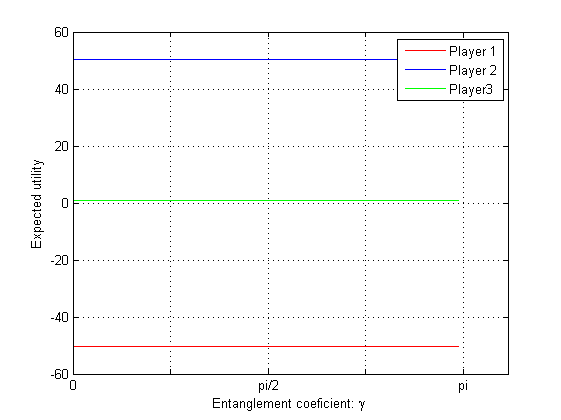
\includegraphics[scale=0.46]{3Rejected99/CDD_CD.PNG}}
    & c1)\putindeepbox[7pt]{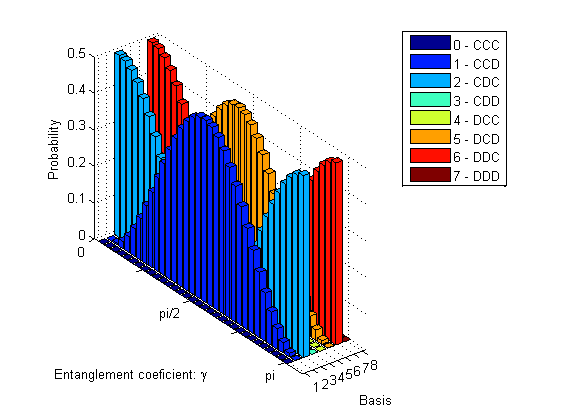
\includegraphics[scale=0.46]{3Rejected99/CDD_CD1.PNG}} \\
\end{tabular}
\caption{Expected utility for $3$ players, where the players will use the $(Cooperate , Defect, Defect)$ operators in the first round of the game; in the second round player 2 and player 3 will play $(CD)$.}
\label{repro:3}
\end{center}
 \end{table}

If in the quantum game the player $1$ decides to defect $D$ and the proposal is rejected we get $4$ different probability distributions that are permuted given the players chosen operators. In Tables \ref{tab:3playerDCD_DC99}, 
\ref{tab:3playerDDC_CD99}, and \ref{tab:3playerDDD_CC99} (in Apendix \ref{ap:d})

In Table \ref{tab:3playerDCD_DC99}, the player $2$ has assumes the strategy $\tau_{2}=(C,D)$, this means that she will play $C$ on the first stage and $D$ on the second stage; In Table \ref{tab:3playerDDC_CD99} her strategy is $\tau_{2}=DC$. As the multiplication by a identity matrix is commutative, in the previous cases, we applied the same operation to player $2$ qubit. This result happens because the players are manipulating their qubits with permutation operators $C$ and $D$; described on Section \ref{subsec:strategic_space}, where we define the strategic space the players have access.

When the parameter $\gamma$ influences the expected utility for the players, we verify the functions that describe the expected utility for player $1$ and $3$ tend have maxima and minima for the same values of $\gamma$. However if player $1$ decides to $Defect$ the two functions will not be synchronized.
The function that describes the expected utility for player $2$ tends to have opposite behaviour. This happens because the captain bribed player $3$ with one gold coin.


\end{comment}



















\subsubsection{The captain proposes: $(100, 0, 0)$}
\label{subsubsec:3playergame100}

Suppose captain is greedy and proposes to get the 100 coins. In the classical Pirate Game this would pose a conflict with his self-preserving needs. 
A pertinent question would be if this Quantum Model of the Pirate Game would allow the first captain to approve that allocation proposal. 

If the captain is the only one with access to quantum strategies, and the other players do not know it and play the classical strategies $C$ (identity matrix) and $D$ (Bit-flip operator), there is a dominant quantum strategy that allows her to pass her proposal and get all the $100$ coins, for $\gamma = \frac{\pi}{2}$. Figure \ref{fig:pg_3players_99_0_1:4} provides an example that corroborates where we verify that player $1$ has a set of dominant strategies (for $\tau_{1} = \mathcal{U}_{1}(\pi,\phi), \phi \in (0, \frac{\pi}{2})$ or $\tau_{1} = \mathcal{U}_{1}(\theta,\frac{\pi}{2}), \theta \in (0, \pi)$). We verified experimentaly that the sub-games with $2$ players (when $(C_{4},C_{5}), (C_{4},D_{5}), (D_{4},C_{5}), (D_{4},D_{5})$), did not affect this dominat strategy. If fact if we analise the expected utility function for player $1$ ($E_{1}.$), and the Figure \ref{fig:pg_architecturegametree:extensiveform} representing the extensive form game, we verify that the the first captain is indiferent to the results of the sub-game with $2$-players, when both player play a classical strategy, because she is already dead. 

\begin{figure}[h]
\centering 
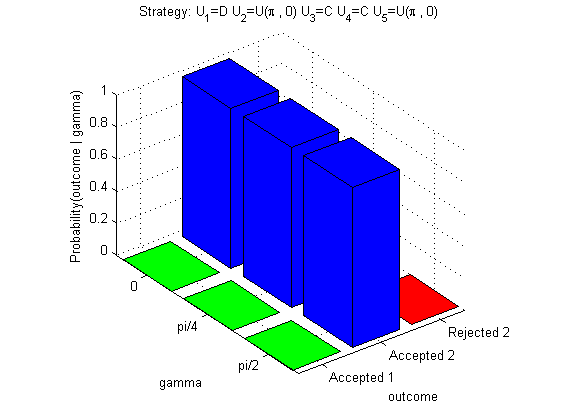
\includegraphics[scale=0.80]{Figures/1.5qubit/DUpi0CCUpi0.png}
\caption{Player $1$ uses the classical operator D. The probabilities don't change with the entanglement.  }
\label{fig:pg_3players_99_0_1:2}
\end{figure}

\begin{figure}[h]
\centering 
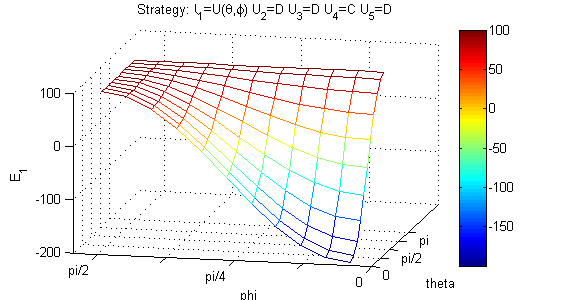
\includegraphics[scale=0.80]{Figures/1.5qubit/meanpirate.png}
\caption{Expected utility for player $1$ when she addopts a strategic move of the form $U_{1}(\theta,\phi)$ and the other players play $D_{2},D_{3},C_{4},D_{5}$. }
\label{fig:pg_3players_99_0_1:4}
\end{figure}

If players $2$ and $3$ know that the captain has access to quantum strategies, with a maximaly entangled game, and they have the restricted sub-set of pure classical strategies $C_{j}$ and $D_{j}$, if they both play $C$, the dominant strategy for the captain becomes $\tau_{1} = \mathcal{U}_{1}(0,0)$. Their best response becomes playing a mixed strategy where half the time they will play $C$ and the other half $D$. The best response for player $1$ in this case is to play a mixed quantum strategy where half the time she plays $\mathcal{U}(0,0)$, half $\mathcal{U}(0,pi/2)$.



\begin{figure}[h]
\centering 
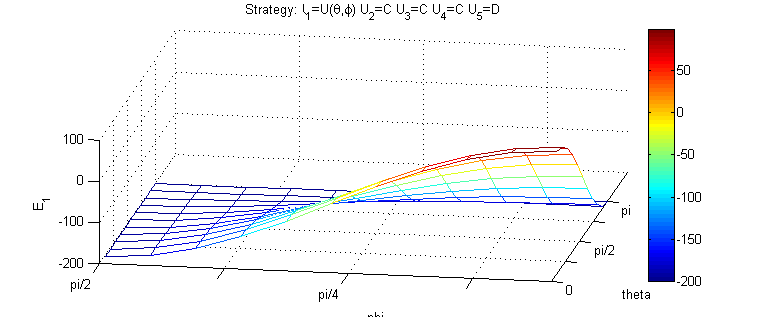
\includegraphics[scale=0.80]{Figures/1.5qubit/meanpirategetscrewed.png}
\caption{Players $2$ and $3$ use a mixed classical strategy to choose the operators $O_{2}$ and $O_{3}$, where half the time they will play $C$ and the other half $D$. }
\label{fig:pg_3players_99_0_1:2}
\end{figure}

\begin{figure}[h]
\centering 
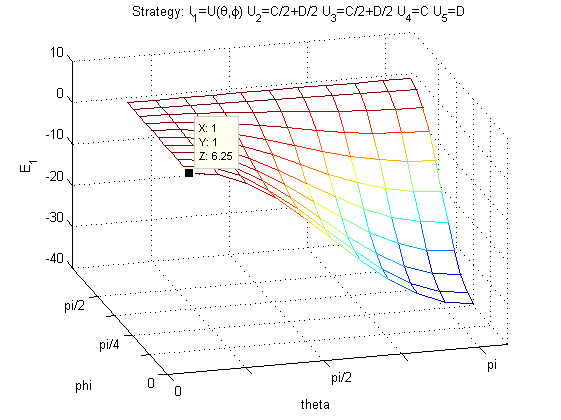
\includegraphics[scale=0.80]{Figures/1.5qubit/mixedclassical.png}
\caption{Players $2$ and $3$ use the operators $C_{2}$ and $C_{3}$. }
\label{fig:pg_3players_99_0_1:2}
\end{figure}

\begin{figure}[h]
\centering 
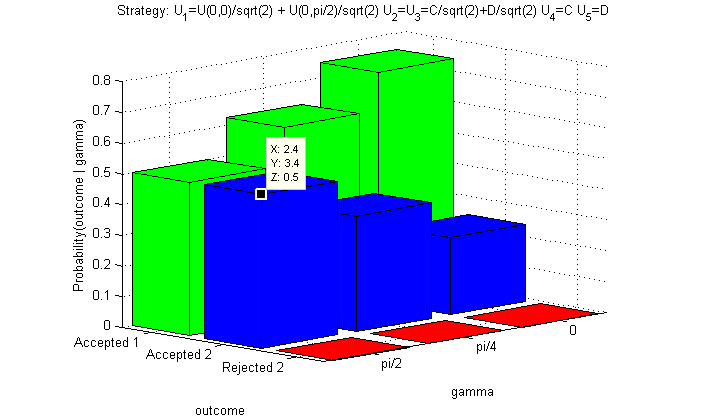
\includegraphics[scale=0.80]{Figures/1.5qubit/mixedmixedclassical.png}
\caption{Players $2$ and $3$ use the operators $C_{2}$ and $C_{3}$. }
\label{fig:pg_3players_99_0_1:2}
\end{figure}




\begin{comment}


The player $1$, the captain, needs two votes to pass her proposal. In order to answer our question we must analyse the expected utilities for all players where the initial proposal is accepted. Moreover we need to analyse an instance where the proposal is refused, when the players select the actions $(C,D,D)$. In the previous analysis we observed that player $2$ has a strong motivation to Defect in the first round, because in the second round she can pass the proposal with her vote alone, this means if the player $1$ wants to pass is proposal she should choose the $C$ operator.

 Our final state will be calculated as shown in Equation \ref{eq:piratas_final_move2_99anal}.



In Table \ref{tab:3playerDCC100} we notice that player $3$ will get a expected payoff of $0.5$ if she chooses to Defect.
\begin{table}[h]
\begin{center}
\begin{tabular}{cc}
  \putindeepbox[7pt]{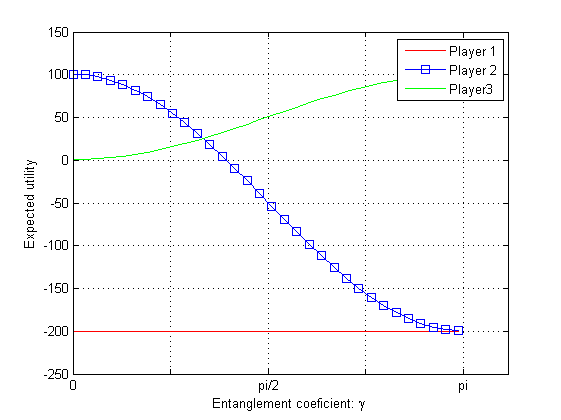
\includegraphics[scale=0.72]{3Accepted100/CDD_CC.PNG}}
\end{tabular}
\caption{Expected utility for $3$ players, where the players will use the $(Cooperate, Defect, Defect)$ operators in the first stage. In the second stage we represented the sub-game equilibrium of the game.  }
\label{tab:3playerDCC100}
\end{center}
 \end{table}


In Tables \ref{tab:3playerCDC100} and \ref{tab:3playerCCD100}, the expected utility function for player $3$ starts of as $0$ for $\gamma=0$ (which corresponds to the classical problem). The function presents a maximum when the system is maximally entangled; this maximum is $0.5$. If the proposal is accepted when the entanglement coefficient is $\gamma=\frac{\pi}{2}$ player $1$ will get a negative expected payoff (which means he will die under that condition).

\begin{table}[h]
\begin{center}
\begin{tabular}{c}
  \putindeepbox[7pt]{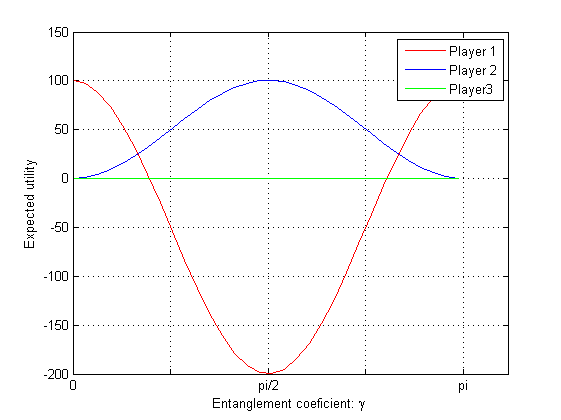
\includegraphics[scale=0.72]{3Accepted100/CCD.PNG}}
\end{tabular}
\caption{Expected utility for $3$ players, where the players will use the $(Cooperate, Cooperate, Defect)$ operators. }
\label{tab:3playerCCD100}
\end{center}
 \end{table}

\begin{table}[h]
\begin{center}
\begin{tabular}{c}
  \putindeepbox[7pt]{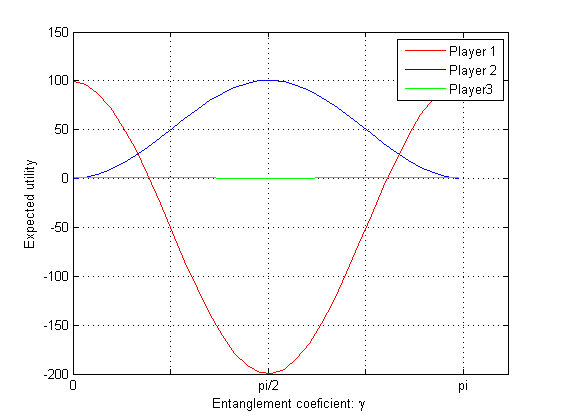
\includegraphics[scale=0.72]{3Accepted100/CDC.PNG}}
   
\end{tabular}
\caption{Expected utility for $3$ players, where the players will use the $(Cooperate, Defect, Cooperate)$ operators.}
\label{tab:3playerCDC100}
\end{center}
 \end{table}

The Table \ref{tab:3playerCCC100} presents an outcome where all the players vote in favour of the proposal. The players $2$ and $3$ have and expected utility of $0$, regardless the role of entanglement in the system.



\begin{table}[h]
\begin{center}
\begin{tabular}{c}
  \putindeepbox[7pt]{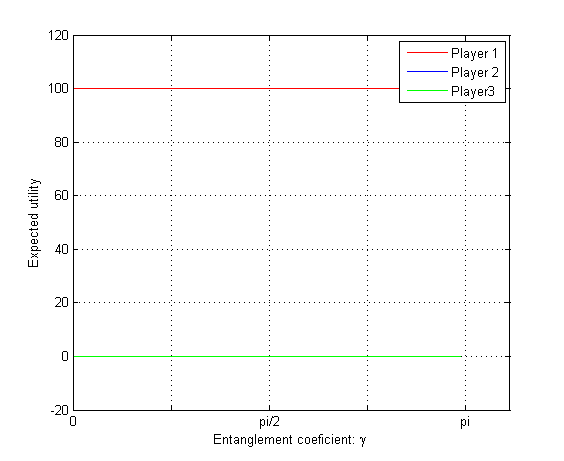
\includegraphics[scale=0.72]{3Accepted100/CCC.PNG}}
\end{tabular}
\caption{Expected utility for $3$ players, where the players will use the $(Cooperate, Cooperate, Cooperate)$ operators. The initial proposal is $(\alpha_{1}, \alpha_{2}, \alpha_{3}) =(100, 0, 0)$. }
\label{tab:3playerCCC100}
\end{center}
 \end{table}

From this simulation we can conclude that if the captain wants to pass her proposal for $\gamma=\frac{\pi}{2}$ there are $3$ equilibria when the player select the operators $(CDC)$, $(C,C,D)$, and $((C,D,D),(C,C))$. $(CDC)$, $(C,C,D)$ correspond to an accepted proposal. However player $1$ will get a negative payoff in any of this equilibria. 

We can interpret this in the context of the problem with the captain getting the coins as she proposed, but being immediately betrayed and killed by her fellow pirates who conspired in order for player $2$ to get all the coins, and player $3$ to become second in command.

Otherwise there is one Nash Equilibrium when the players select $((C,D,D),(C,C))$. Even in a quantum version, the captain needs to bribe player $3$ in order to approve her proposal and get a maximum of $99$ gold coins.


\end{comment}




